%%%%%%%%%%%%%%%%%%%%%%%%%%%%%%%%%%%%%%%%%%%%%%%%%%%%%%%%%%%%%%%
%%% HEADER %%%%%%%%%%%%%%%%%%%%%%%%%%%%%%%%%%%%%%%%%%%%%%%%%%%%
%%%%%%%%%%%%%%%%%%%%%%%%%%%%%%%%%%%%%%%%%%%%%%%%%%%%%%%%%%%%%%%

\documentclass{layout/si-msc-proposal}
\usepackage{float}
\usepackage{todonotes}
\usepackage{dirtytalk}
\usepackage{subcaption}
\usepackage{listings}
\usepackage{tikz}
\usepackage{color}
\usepackage{pgfgantt}
\usepackage{hyperref}

\graphicspath{ {./images/} }

\newcommand\YAMLcolonstyle{\color{red}\mdseries}
\newcommand\YAMLkeystyle{\color{black}\bfseries}
\newcommand\YAMLvaluestyle{\color{blue}\mdseries}

\makeatletter

\newcommand\language@yaml{yaml}

\expandafter\expandafter\expandafter\lstdefinelanguage
\expandafter{\language@yaml}
{
    keywords={true,false,null,y,n},
    keywordstyle=\color{darkgray}\bfseries,
    basicstyle=\YAMLkeystyle,
    sensitive=false,
    comment=[l]{\#},
    morecomment=[s]{/*}{*/},
    commentstyle=\color{purple}\ttfamily,
    stringstyle=\YAMLvaluestyle\ttfamily,
    moredelim=[l][\color{orange}]{\&},
    moredelim=[l][\color{magenta}]{*},
    moredelim=**[il][\YAMLcolonstyle{:}\YAMLvaluestyle]{:},
    morestring=[b]',
    morestring=[b]",
    literate =    {---}{{\ProcessThreeDashes}}3
        {>}{{\textcolor{red}\textgreater}}1
        {|}{{\textcolor{red}\textbar}}1
        {\ -\ }{{\mdseries\ -\ }}3,
}

\setlength\parindent{0pt}

\author{Edoardo Riggio}

\title{API Scout: An Information Retrieval System for OpenAPI Specifications}

\abstract{

    The primary objective of this thesis is to create an information retrieval system enabling users to explore a comprehensive collection of OpenAPI specifications. The system will use historical versioned data - scraped from existing github repositories - as well as user-uploaded data. \\

    This platform serves a dual purpose, catering to both academics and developers. In the case of academics, this platform can serve as a repository from which to conduct research, facilitating more in-depth studies on API specifications and their evolution. On the other hand, developers can look up several different examples that could help them get started with their own OpenAPI documentation. \\

    The main contributions of this thesis include two crucial aspects: data engineering and software engineering. In the first case, the thesis will delve in the process of refining raw data and finding ways to classify the API specifications. In the second case, the thesis will define the architectural design and the development of the service itself.

}

\begin{document}

    \maketitle

%%%%%%%%%%%%%%%%%%%%%%%%%%%%%%%%%%%%%%%%%%%%%%%%%%%%%%%%%%%%%%%
%%% MAIN BODY %%%%%%%%%%%%%%%%%%%%%%%%%%%%%%%%%%%%%%%%%%%%%%%%%
%%%%%%%%%%%%%%%%%%%%%%%%%%%%%%%%%%%%%%%%%%%%%%%%%%%%%%%%%%%%%%%

    \tableofcontents
    \listoffigures
    \listoftables
    \newpage

%%%%%%%%%%%%%%%%%%%%%%%%%%%%%%%%%%%%%%%%%%%%%%%%%%%%%%%%%%%%%%%
%%%%%%%%%%%%%%%%%%%%%%%%%%%%%%%%%%%%%%%%%%%%%%%%%%%%%%%%%%%%%%%

    \section{Introduction}\label{sec:introduction}

    \subsection{Context}\label{subsec:context}
    \input{sections/introduction/context}

    \subsection{Motivation}\label{subsec:motivation}
    From our research, we noticed that there is a void in tools and services that can be helpful in the study of the evolution and current state of HTTP APIs.
Although platforms such as SwaggerHub\footnote{https://app.swaggerhub.com/search} and APIs.guru\footnote{https://apis.guru/} already exist, they lack features that are essential for research. \\ \\
For example, they lack a proper search system.
In the previously mentioned platforms, indexing of specifications is superficial and most of the time only the title is matched with the query.
With API Scout, we want to index API specifications based not only on their title, but based on all the tags containing natural language. \\ \\
Another feature missing in the aforementioned platforms is a proper visualization system.
By using tools to convert specifications into interactive trees, users can better understand the structure of the service's endpoints.
Moreover, we can also plot some statistics about the selected API and how it compares to all the specifications present on our platform.

    \subsection{Objective}\label{subsec:objective}
    The goal of this thesis is to build a platform that both academics and developers can use to understand and study the intricacies of real-world HTTP APIs. \\ \\
In the case of the developers, they can search and consult our historical and current collection of APIs to better understand how to structure one.
Aided by the graphical tools, a developer can also understand how the endpoints should be structured to obtain a more cohesive structure. \\ \\
On the academic side, this tool can be used to perform research on the evolution of HTTP APIs in time.
By offering historical data as well as current data, researchers can have a better understanding of how endpoints and data structures change over time as a service grows in complexity.
Researchers can also use plots and statistics pre-computed by our platform to understand how an API specification relates to the plethora of specifications present.

%%%%%%%%%%%%%%%%%%%%%%%%%%%%%%%%%%%%%%%%%%%%%%%%%%%%%%%%%%%%%%%
%%%%%%%%%%%%%%%%%%%%%%%%%%%%%%%%%%%%%%%%%%%%%%%%%%%%%%%%%%%%%%%

    \section{Proposal}\label{sec:proposal}


    \section{State of the Art}\label{sec:state-of-the-art}


    \section{Preliminary Results - Feasibility Study}\label{sec:preliminary-results---feasibility-study}


    \section{Work Plan for the Spring semester}\label{sec:work-plan-for-the-spring-semester}
    This section describes a high level view of the work plan for the spring semester.

\begin{itemize}
    \item Iteration 1: Data Analysis Phase
    \begin{itemize}
        \item Task 1: Setup project (Pick tools/technologies to use)
        \item Task 2: Design of metrics to locate changes in evolution
        \item Task 3: Setup database of metrics
        \item Task 4: Classification of changes
        \item Task 5: Evaluate and improve system
    \end{itemize}
    \item Iteration 2: Visualization Phase
    \begin{itemize}
        \item Task 1: High level visualization of API
        \item Task 2: Drilled down visualization of API
        \item Task 3: Visualizing changes
        \item Task 4: Evaluate and improve system
    \end{itemize}
    \item Iteration 3: Report
\end{itemize}
\resizebox{\textwidth}{!}{
    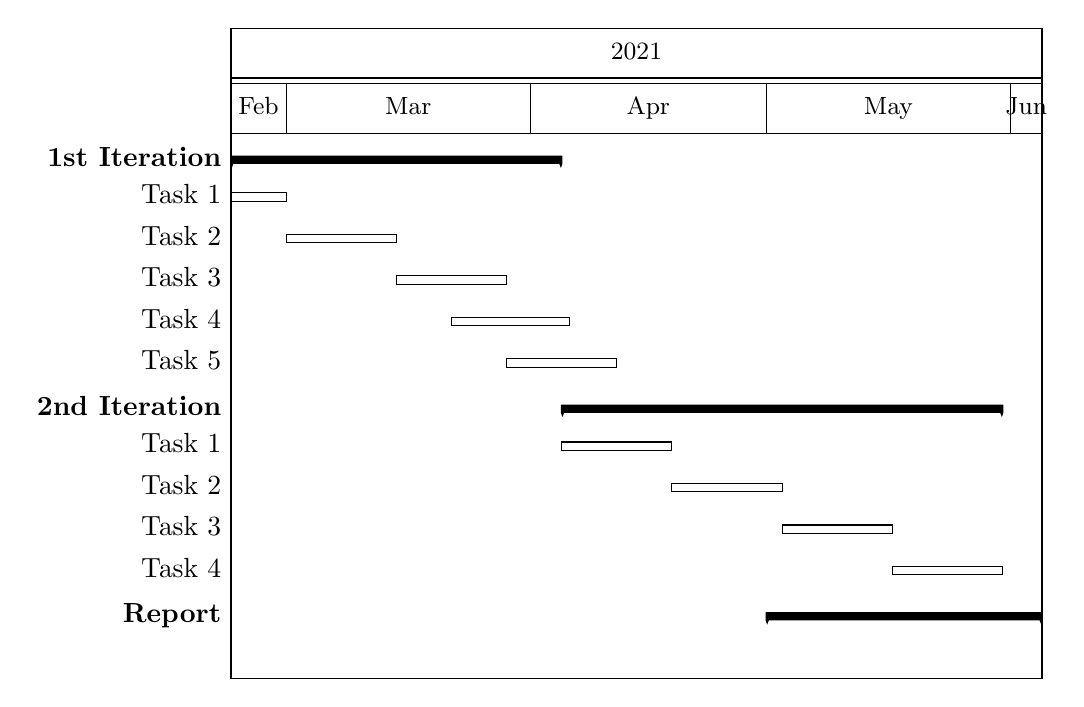
\begin{tikzpicture}
        \begin{ganttchart}[
            Mile1/.style={milestone/.append style={fill=red}},
            x unit=1mm,
            time slot format=isodate,
            y unit title=20,
            title height=.9,
            bar height=0.2,
            y unit chart=15,
        ]
        {2021-2-22}{2021-6-4}

            \gantttitlecalendar{year, month=shortname} \\

            \ganttgroup{1st Iteration}{2021-2-22}{2021-4-4} \\
            \ganttbar{Task 1}{2021-2-22}{2021-2-28}\\
            \ganttbar{Task 2}{2021-2-29}{2021-3-14}\\
            \ganttbar{Task 3}{2021-3-15}{2021-3-28}\\
            \ganttbar{Task 4}{2021-3-22}{2021-4-5}\\
            \ganttbar{Task 5}{2021-3-29}{2021-4-11}\\
            \ganttgroup{2nd Iteration}{2021-4-5}{2021-5-30} \\
            \ganttbar{Task 1}{2021-4-5}{2021-4-18}\\
            \ganttbar{Task 2}{2021-4-19}{2021-5-2}\\
            \ganttbar{Task 3}{2021-5-3}{2021-5-16}\\
            \ganttbar{Task 4}{2021-5-17}{2021-5-30}\\
            \ganttgroup{Report}{2021-5-1}{2021-6-4} \\
        \end{ganttchart}
    \end{tikzpicture}
}


%%%%%%%%%%%%%%%%%%%%%%%%%%%%%%%%%%%%%%%%%%%%%%%%%%%%%%%%%%%%%%%
%%% BIBLIOGRAPHY %%%%%%%%%%%%%%%%%%%%%%%%%%%%%%%%%%%%%%%%%%%%%%
%%%%%%%%%%%%%%%%%%%%%%%%%%%%%%%%%%%%%%%%%%%%%%%%%%%%%%%%%%%%%%%

    \newpage
    \nocite{*}
    \bibliographystyle{unsrt}
    \bibliography{bibliography/bibliography}%

\end{document}